\chapter{هندسه‌ی مسطحه}
\thispagestyle{empty}

\begin{quote}
	{\lotus
		اقلیدس به من آموخت که بدون فرضیات، هیچ برهانی وجود ندارد. بنابراین، در هر استدلالی، فرضیات را بیازمایید. \quad - بل%
		\LTRfootnote{ Eric Temple Bell}
	}
\end{quote}

\section{تعریف‌ها و اصول اولیه}
\textbf{نقطه:}
از مفاهیم تعریف‌نشده است. نقطه را معمولاً با یک حرف بزرگ نشان می‌دهند؛ مانند نقطه‌ی $A$.
\begin{example}
	نقطه‌ی $A$:
	\begin{center}
		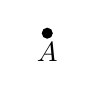
\begin{tikzpicture}
			\centering
			\fill (0,0) circle (2pt) node[below] {$A$};
		\end{tikzpicture}
	\end{center}
\end{example}
\smallskip
\textbf{خط راست:}
از مفاهیم تعریف‌نشده است. خط با دو نقطه‌ی متمایز از آن و گاهی با یک حرف کوچک نمایش داده می‌شود؛ مانند خط $AB$ یا خط $d$.
\begin{example}
	خط
	$\ell$:
	\begin{center}
		\begin{tikzpicture}
			\draw[thick] (-2,0) -- (3,0) node[below] {$\ell$};
		\end{tikzpicture}
	\end{center}
\end{example}
\smallskip
\textbf{نیم‌خط راست:}
مجموعه‌ای از نقطه‌های خط راست است که در یک طرف نقطه‌ی ثابتی از آن خط راست قرار دارد. این نقطه‌ی ثابت را مبدأ نیم‌خط می‌نامند؛ مانند نیم‌خط $Ox$.
\begin{example}
	نیم‌خط $Ox$:
	\begin{center}
		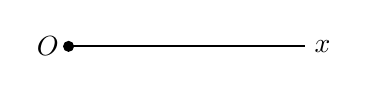
\begin{tikzpicture}
			\draw[thick] (0,0) -- (3,0);
			\fill (0,0) circle (2pt) node[left] {$O$};
			\node[right] at (3,0) {$x$};
		\end{tikzpicture}
	\end{center}
\end{example}
\smallskip
\textbf{پاره‌خط راست:}
بخشی از یک خط راست است که از دو طرف به دو نقطه محدود باشد؛ مانند پاره‌خط $AB$.
\begin{example}
	پاره‌خط $AB$:
	\begin{center}
		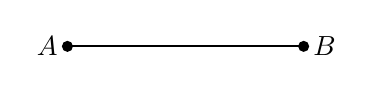
\begin{tikzpicture}
			\draw[thick] (0,0) -- (3,0);
			\fill (0,0) circle (2pt) node[left] {$A$};
			\fill (3,0) circle (2pt) node[right] {$B$};
		\end{tikzpicture}
	\end{center}
\end{example}
\begin{example}
	روی خط راستی، ۵۰ پاره‌خط راست داده شده است. ثابت کنید دست‌کم یکی از دو حکم زیر درست است:
	\begin{enumerate}
		\item 
		هشت پاره‌خط راست پیدا می‌شود که دارای نقطه‌ی مشترکی هستند.
		\item 
		هشت پاره‌خط راست وجود دارد که هیچ دوتایی از آن‌ها نقطه‌ی مشترکی ندارند.
	\end{enumerate}
	\textbf{پاسخ:}
\end{example}
\smallskip
\textbf{زاویه:}
شکلی است که از دو نیم‌خط با مبدأ مشترک پدید می‌آید. مبدأ مشترک، رأس زاویه و هر یک از دو نیم‌خط یک ضلع زاویه نامیده می‌شود؛ مانند زاویه‌ی $xOy$. گاهی زاویه را فقط با حرف رأس آن نمایش می‌دهند؛ مانند زاویه‌ی $O$. گاهی هم از یک حرف که در مجاورت رأس و بین دو ضلع نوشته می‌شود، استفاده می‌شود؛ مانند زاویه‌ی
$\alpha$.
زاویه را با نماد
$\angle$
نشان می‌دهند، مانند
$\angle xOy$.
\begin{example}
	زاویه‌ی $xOy$:
	\begin{center}
		\begin{tikzpicture}
			\coordinate (O) at (0,0);
			\coordinate (x) at (3,0);
			\coordinate (y) at (2,2.5);
			\draw[thick] (O) -- (x) node[right] {$x$};
			\draw[thick] (O) -- (y) node[right] {$y$};
			\fill (O) circle (2pt) node[below left] {$O$};
			\pic[draw, angle eccentricity=1.6, angle radius=0.8cm] {angle = x--O--y};
		\end{tikzpicture}
	\end{center}
\end{example}
\smallskip
\textbf{زاویه‌ی نیم‌صفحه:}
زاویه‌ای است که دو ضلع آن در یک امتداد باشند.
\begin{example}
	زاویه‌ی نیم‌صفحه‌ی $xOy$:
	\begin{center}
		\begin{tikzpicture}
			\coordinate (O) at (0,0);
			\coordinate (x) at (2,0);
			\coordinate (y) at (-2,0);
			\draw[thick] (O) -- (x) node[right] {$x$};
			\draw[thick] (O) -- (y) node[left] {$y$};
			\fill (O) circle (2pt) node[below] {$O$};
			\pic[draw, angle eccentricity=1.6, angle radius=0.5cm] {angle = x--O--y};
		\end{tikzpicture}
	\end{center}
\end{example}
\smallskip
\textbf{نیمساز زاویه:}
نیم‌خطی است که مبدأ آن رأس زاویه است و زاویه را به دو زاویه‌ی مساوی تقسیم می‌کند.
\begin{example}
	نیم‌خط $OC$ نیمساز زاویه‌ی $AOB$ است؛ یعنی
	$\angle AOC = \angle BOC$.
	\begin{center}
		\begin{tikzpicture}
			\coordinate (O) at (0,0);
			\coordinate (A) at (3,0);
			\coordinate (B) at (2.5,2);
			\coordinate (C) at (2.8,1);
			\draw[thick] (O) -- (A) node[right] {$A$};
			\draw[thick] (O) -- (B) node[right] {$B$};
			\draw[thick] (O) -- (C) node[right] {$C$};
			\fill (O) circle (2pt) node[below left] {$O$};
			\pic[draw, angle eccentricity=1.5, angle radius=0.5cm] {angle = A--O--C};
			\pic[draw, angle eccentricity=1.5, angle radius=0.5cm] {angle = C--O--B};
		\end{tikzpicture}
	\end{center}
\end{example}
\begin{theorem}
	هر زاویه فقط یک نیمساز دارد.
	\\ \dfth \\
	\textbf{برهان:}
	اگر $Oz$ و $Ot$ هر دو نیمساز
	$\angle xOy$
	باشند، داریم:
	\[
	\begin{rcases}
		\angle xOz = \frac{1}{2} \angle xOy \\
		\angle xOt = \frac{1}{2} \angle xOy
	\end{rcases}
	\Rightarrow \angle xOz = \angle xOt
	\]
چون این دو زاویه‌ی مساوی در رأس $O$ و در ضلع $Ox$ مشترکند و در یک طرف آن ضلع قرار دارند، الزاماً دو ضلع دیگر آن‌ها بر هم منطبق می‌شوند. پس
$\angle xOy$
فقط یک نیمساز دارد.
\qed
\end{theorem}
\smallskip
\textbf{اندازه‌ی زاویه:}
نسبت آن زاویه است به زاویه‌ای که به عنوان واحد اختیار شده است.
\\
\textbf{واحد اندازه‌گیری زاویه:}
واحدی است که به‌کمک آن می‌توان اندازه‌ی زاویه‌ها را تعیین کرد. یکی از واحدهای اندازه‌گیری زاویه،
\textbf{درجه}
است که
$\frac{1}{180}$
زاویه‌ی نیم‌صفحه است. علامت درجه
$\circ$
است، مثلاً
$\ang{180}$
را ۱۸۰ درجه می‌خوانیم.
یکی دیگر از واحدهای اندازه‌گیری زاویه،
\textbf{رادیان}
است که
$\frac{1}{\pi}$
زاویه‌ی نیم‌صفحه است. اگر اندازه‌ی یک زاویه را برحسب درجه با $D$ و برحسب رادیان با $R$ نمایش دهیم، بین $D$ و $R$ رابطه‌ی
$\frac{D}{180}=\frac{R}{\pi}$
برقرار است.
\begin{example}
	زاویه‌ی
	$\frac{\pi}{3}$
	رادیان برابر با
	$\ang{60}$
	است.
\end{example}
\smallskip
\textbf{زاویه‌ی قائمه:}
نصف زاویه‌ی نیم‌صفحه است. اندازه‌ی زاویه‌ی قائمه برابر ۹۰ درجه یا
$\frac{\pi}{2}$
رادیان است. زاویه‌ی قائمه را زاویه‌ی راست نیز می‌نامند.
\begin{example}
	زاویه‌ی قائمه‌ی $xOy$:
	\begin{center}
		\begin{tikzpicture}
			\coordinate (O) at (0,0);
			\coordinate (x) at (2,0);
			\coordinate (y) at (0,2);
			\draw[thick] (O) -- (x) node[right] {$x$};
			\draw[thick] (O) -- (y) node[left] {$y$};
			\fill (O) circle (2pt) node[below] {$O$};
			\pic[draw, angle eccentricity=1.6, angle radius=0.5cm] {angle = x--O--y};
		\end{tikzpicture}
	\end{center}
\end{example}
\smallskip
\textbf{زاویه‌ی تند (حاده):}
زاویه‌ای است که از زاویه‌ی قائمه کوچک‌تر است. اندازه‌ی زاویه‌ی تند بین صفر و ۹۰ درجه است.
\begin{example}
	زاویه‌ی تند (حاده) $xOy$:
	\begin{center}
		\begin{tikzpicture}
			\coordinate (O) at (0,0);
			\coordinate (x) at (2,0);
			\coordinate (y) at (1.7,1.5);
			\draw[thick] (O) -- (x) node[right] {$x$};
			\draw[thick] (O) -- (y) node[left] {$y$};
			\fill (O) circle (2pt) node[below] {$O$};
			\pic[draw, angle eccentricity=1.6, angle radius=0.5cm] {angle = x--O--y};
		\end{tikzpicture}
	\end{center}
\end{example}
\smallskip
\textbf{زاویه‌ی باز (منفرجه):}
زاویه‌ای است بزرگ‌تر از زاویه‌ی قائمه و کوچک‌تر از زاویه‌ی نیم‌صفحه. اندازه‌ی زاویه‌ی باز بین ۹۰ درجه و ۱۸۰ درجه است.
\begin{example}
	زاویه‌ی باز (منفرجه) $xOy$:
	\begin{center}
		\begin{tikzpicture}
			\coordinate (O) at (0,0);
			\coordinate (x) at (2.5,0);
			\coordinate (y) at (-2,1.5);
			\draw[thick] (O) -- (x) node[right] {$x$};
			\draw[thick] (O) -- (y) node[left] {$y$};
			\fill (O) circle (2pt) node[below] {$O$};
			\pic[draw, angle eccentricity=1.6, angle radius=0.5cm] {angle = x--O--y};
		\end{tikzpicture}
	\end{center}
\end{example}
\smallskip
\textbf{زاویه‌ی صفر:}
زاویه‌ای است که دو ضلع آن بر هم منطبق‌اند.
\begin{example}
	زاویه‌ی صفر $xOy$:
	\begin{center}
		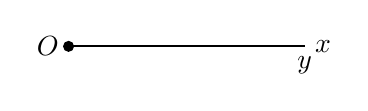
\begin{tikzpicture}
			\coordinate (O) at (0,0);
			\coordinate (x) at (3,0);
			\coordinate (y) at (3,0);
			\draw[thick] (O) -- (x) node[below] {$y$};
			\draw[thick] (O) -- (y) node[right] {$x$};
			\fill (O) circle (2pt) node[left] {$O$};
		\end{tikzpicture}
	\end{center}
\end{example}
\smallskip
\textbf{زاویه‌ی کوژ (محدب):}
زاویه‌ای است که از زاویه‌ی نیم‌صفحه کوچک‌تر است. اندازه‌ی زاویه‌ی کوژ بین صفر و ۱۸۰ درجه است.
\\
\textbf{زاویه‌ی کاو (مقعر):}
زاویه‌ای است که از زاویه‌ی نیم‌صفحه بزرگ‌تر است. اندازه‌ی زاویه‌ی کاو از ۱۸۰ درجه بیشتر است.
\begin{example}
	زاویه‌ی کاو $xOy$:
	\begin{center}
		\begin{tikzpicture}
			\coordinate (O) at (0,0);
			\coordinate (x) at (2.5,0);
			\coordinate (y) at (-2,-1.5);
			\draw[thick] (O) -- (x) node[right] {$x$};
			\draw[thick] (O) -- (y) node[left] {$y$};
			\fill (O) circle (2pt) node[below] {$O$};
			\pic[draw, angle eccentricity=1.6, angle radius=0.5cm] {angle = x--O--y};
		\end{tikzpicture}
	\end{center}
\end{example}
\smallskip
\textbf{دو زاویه‌ی مجاور:}
دو زاویه‌ای هستند که در رأس و یک ضلع مشترکند و دو ضلع غیرمشترک آن‌ها در دو طرف ضلع مشترکشان قرار دارد.
\begin{example}
	دو زاویه‌ی $AOC$ و $BOC$ مجاور (همسایه) هستند.
	\begin{center}
		\begin{tikzpicture}
			\coordinate (O) at (0,0);
			\coordinate (A) at (3,0);
			\coordinate (B) at (2.5,2.5);
			\coordinate (C) at (2.8,1);
			\draw[thick] (O) -- (A) node[right] {$A$};
			\draw[thick] (O) -- (B) node[right] {$B$};
			\draw[thick] (O) -- (C) node[right] {$C$};
			\fill (O) circle (2pt) node[below left] {$O$};
			\pic[draw, angle eccentricity=1.5, angle radius=0.5cm] {angle = A--O--C};
			\pic[draw, angle eccentricity=1.5, angle radius=0.5cm] {angle = C--O--B};
		\end{tikzpicture}
	\end{center}
\end{example}
\smallskip
\textbf{دو زاویه‌ی متمم:}
دو زاویه‌ای هستند که مجموع آن‌ها یک زاویه‌ی قائمه است. به بیان دیگر، مجموع اندازه‌های آن‌ها برابر ۹۰ درجه است. دو زاویه‌ی متمم لزوماً مجاور نیستند.
\begin{example}
	دو زاویه‌ی
	$\ang{40}$ و $\ang{50}$
	متمم یکدیگر هستند.
\end{example}
\smallskip
\textbf{دو زاویه‌ی مکمل:}
دو زاویه‌ای هستند که مجموع آن‌ها یک زاویه‌ی نیم‌صفحه است. به بیان دیگر، مجموع اندازه‌های آن‌ها برابر ۱۸۰ درجه است. دو زاویه‌ی مکمل لزوماً مجاور نیستند.
\begin{example}
	دو زاویه‌ی
	$\ang{110}$ و $\ang{70}$
	مکمل یکدیگر هستند.
\end{example}
\smallskip
\textbf{دو زاویه‌ی مجانب:}
دو زاویه‌ای هستند که مکمل و مجاورند.
\begin{example}
	دو زاویه‌ی $AOC$ و $BOC$ مجانب هستند.
	\begin{center}
		\begin{tikzpicture}
			\coordinate (O) at (0,0);
			\coordinate (A) at (2.5,0);
			\coordinate (B) at (-2.5,0);
			\coordinate (C) at (2,1);
			\draw[thick] (O) -- (A) node[right] {$A$};
			\draw[thick] (O) -- (B) node[left] {$B$};
			\draw[thick] (O) -- (C) node[right] {$C$};
			\fill (O) circle (2pt) node[below] {$O$};
			\pic[draw, angle eccentricity=1.5, angle radius=0.5cm] {angle = A--O--C};
			\pic[draw, angle eccentricity=1.5, angle radius=0.5cm] {angle = C--O--B};
		\end{tikzpicture}
	\end{center}
\end{example}
\smallskip
\textbf{دو زاویه‌ی متقابل به رأس:}
دو زاویه را که رأس مشترک داشته باشند و ضلع‌های آن‌ها دوبه‌دو در امتداد یکدیگر و در جهت‌های مخالف باشند، متقابل به رأس می‌گوییم.
\begin{example} \label{geexmotaberas}
	دو زاویه‌ی $xOy$ و $x'Oy'$ متقابل به رأس هستند.
	\begin{center}
		\begin{tikzpicture}
			\coordinate (O) at (0,0);
			\coordinate (x1) at (2.5,1.5);
			\coordinate (y1) at (2.5,-1.5);
			\coordinate (x2) at (-2.5,-1.5);
			\coordinate (y2) at (-2.5,1.5);
			\draw[thick] (O) -- (x1) node[right] {$x$};
			\draw[thick] (O) -- (y1) node[right] {$y$};
			\draw[thick] (O) -- (x2) node[left] {$x'$};
			\draw[thick] (O) -- (y2) node[left] {$y'$};
			\fill (O) circle (2pt) node[below] {$O$};
			\pic[draw, angle eccentricity=1.5, angle radius=0.5cm] {angle = y1--O--x1};
			\pic[draw, angle eccentricity=1.5, angle radius=0.5cm] {angle = y2--O--x2};
		\end{tikzpicture}
	\end{center}
\end{example}
\begin{theorem}
	دو زاویه‌ی متقابل به رأس مساوی هستند.
	\\ \dfth \\
	\textbf{برهان:}
	دو زاویه‌ی متقابل به رأس $xOy$ و $x'Oy'$ مثال
	\ref{geexmotaberas}
	را در نظر بگیرید. با فرض
	$\angle xOy = \alpha$ و $\angle x'Oy' = \beta$ و $\angle xOy' = \gamma$
	داریم:
	\[
	\begin{cases}
		\angle yOy' = \ang{180} \Rightarrow \alpha + \gamma = \ang{180} \\
		\angle xOx' = \ang{180} \Rightarrow \beta + \gamma = \ang{180}
	\end{cases}
	\Rightarrow \ \alpha = \beta \ \Rightarrow \ \angle xOy = \angle x'Oy'
	\]
	\qed
\end{theorem}
\begin{theorem}
	اگر دو زاویه‌ی مساوی رأس مشترک داشته باشند و یک ضلع از یکی با یک ضلع از دیگری بر امتداد یک خط راست و در دو جهت مخالف باشد و دو ضلع دیگر آن‌ها متمایز با آن خط راست و در دو طرف آن خط راست باشند، دو زاویه‌ی متقابل به رأس تشکیل می‌دهند (یعنی دو ضلع دیگر آن‌ها نیز بر امتداد یک خط راست هستند).
	\\ \dfth \\
	\textbf{برهان:}
	شکل مثال
	\ref{geexmotaberas}
	را در نظر بگیرید. اگر
	$\angle xOy = \angle x'Oy'$
	و $xOx'$ خط راست باشد، می‌خواهیم ثابت کنیم که
	$yOy'$
	نیز خط راست است.  با فرض
	$\angle xOy = \alpha$ و $\angle x'Oy' = \beta$ و $\angle xOy' = \gamma$
	داریم:
	\[
	\begin{rcases}
		\angle xOx' = \ang{180} \Rightarrow \beta + \gamma = \ang{180} \\
		\angle xOy = \angle x'Oy' \ \Rightarrow \ \alpha = \beta
	\end{rcases}
	\Rightarrow \alpha + \gamma = \ang{180} \ \Rightarrow \ \angle xOy + \angle xOy' = \angle yOy' = \ang{180}
	\]
	\qed
\end{theorem}
\begin{theorem}
	نیمسازهای دو زاویه‌ی متقابل به رأس بر یک خط راست واقع هستند.
	\\ \dfth \\
	\textbf{برهان:}
	
\end{theorem}
%%%%%%%%%%%%%%%%%%%%%%%%%%%%%%%%%%%%%%%%%%%%%
\bigskip
\textbf{اصول پنجگانه‌ی اقلیدس:}
\begin{enumerate}
	\item 
	به‌ازای هر نقطه‌ی $P$ و هر نقطه‌ی $Q$ که با $P$ مساوی نباشد، خط یکتایی مانند $L$ وجود دارد که بر $P$ و $Q$ می‌گذرد. (هر دو نقطه‌ی متمایز یک خط راست منحصربه‌فرد را مشخص می‌سازند.)
	\item 
	به‌ازای هر پاره‌خط $AB$ و هر پاره‌خط $CD$، نقطه‌ی منحصربه‌فردی چون $E$ وجود دارد، چنان‌که $B$ میان $A$ و $E$ واقع است و پاره‌خط $CD$ با پاره‌خط $BE$ قابل انطباق است. (هر پاره‌خط $AB$ را می‌توان به اندازه‌ی پاره‌خط $BE$ که با پاره‌خط داده‌شده‌ی $CD$ قابل انطباق است، امتداد داد.)
	\item 
	به‌ازای هر نقطه‌ی $O$ و هر نقطه‌ی $A$ که با $O$ مساوی نباشد، دایره‌ای به مرکز $O$ و به شعاع $OA$ وجود دارد.
	\item 
	همه‌ی زاویه‌های قائمه
	($\ang{90}$)
	با یکدیگر قابل انطباق‌اند (برابرند).
	\item 
	اگر دو خط به‌وسیله‌ی خط موربی چنان قطع شوند که مجموع اندازه‌های دو زاویه‌ی درونی واقع در یک طرف خط مورب کمتر از
	$\ang{180}$
	باشد، اگر این دو خط را بی‌نهایت امتداد دهیم، آنگاه این دو خط همدیگر را در همان طرف خط مورب، قطع می‌کنند.
\end{enumerate}
\smallskip
\textbf{اصل توازی پلی‌فیر:}
به‌ازای هر خط $L$ و هر نقطه‌ی $P$ غیر واقع بر آن، تنها یک خط مانند $m$ وجود دارد چنان‌که از $P$ می‌گذرد و با $L$ موازی است.

\section{مثلث}

\section{چندضلعی‌ها}

\section{دایره}
